\begin{ledgroupsized}[r]{120mm}
\footnotesize
\pstart
\noindent\textbf{\"{U}berlieferung:}
\pend
\end{ledgroupsized}
\begin{ledgroupsized}[r]{114mm}
\footnotesize
\pstart \parindent -6mm
\makebox[6mm][l]{\textit{L}}Konzept: LH XXXV 13, 3 Bl. 261-262 und LH XXXV 14, 2 Bl. 116, 125-126. 2 Bog. und 1 Bl. 2\textsuperscript{o}. 7 S. fortlaufend beschrieben, Textfolge: Bl. 261, 262, 125 und 126~r\textsuperscript{o} (\"{U}bergang von Bl. 262~v\textsuperscript{o} zu Bl. 125~r\textsuperscript{o} sowie von Bl. 125~v\textsuperscript{o} zu Bl. 126~r\textsuperscript{o} inhaltlich begr\"{u}ndet); Bl. 116 und Bl. 126~v\textsuperscript{o} leer. Bl. 261 und 262 sowie Bl. 116 und 126 bilden jeweils einen Bogen; Bl. 125 ist ein eingeschobenes Einzelblatt. Das St\"{u}ck hat weder \"{U}berschrift noch offenbar Anfang. Die Sprache ist abwechselnd Franz\"{o}sisch oder Latein. Der Text wurde editorisch in drei Teile unterteilt, die als verschiedene Redaktionsstufen gedeutet werden k\"{o}nnten. Alle Texttr\"{a}ger weisen den gleichen Wasserzeichentypus auf. \\Cc 2, Nr. 947
\pend
\end{ledgroupsized}
%\normalsize
\vspace*{5mm}
\begin{ledgroup}
\footnotesize 
\pstart
\noindent\footnotesize{\textbf{Datierungsgr\"{u}nde}: Das vorliegende St\"{u}ck ist haupts\"{a}chlich mit der Berechnung der zwei Widerstands\-arten eines Mediums befasst, die in N. ??R/5\textsubscript{4} sowie in den sp\"{a}teren N. ??R/7\textsubscript{1} und ??R/7\textsubscript{2} unterschieden werden. Beide Widerstandsarten -- die nur vom Medium abh\"{a}ngige \textit{r\'{e}sistance absolue} und die zur Geschwindigkeit des beweglichen K\"{o}rpers proportionale \textit{r\'{e}sistance respective} -- werden in N. ??R/6 als Ursachen gleichm\"{a}{\ss}iger Verz\"{o}gerung in Betracht gezogen. N. ??R/6 weist zudem an einer Stelle (S. ??, Z. ??-?? [[262r]]) auf die spezifische Auffassung der Verz\"{o}gerung hin, die in N. ??R/5\textsubscript{3} und ??R/5\textsubscript{4}, sowie in N. ??R/7\textsubscript{1} und ??R/7\textsubscript{2} vorgetragen wird. Letztere vier St\"{u}cke enthalten wiederum Anspielungen, die sich als Verweise auf N. ??R/6 deuten lassen. S\"{a}mtliche Texttr\"{a}ger von N. ??R/6 weisen allerdings den gleichen Wasserzeichentypus wie die Texttr\"{a}ger von N. ??R/5 auf, w\"{a}hrend die sp\"{a}tere N. ??R/7 verschiedene Wasserzeichen hat. Daher wird N. ??R/6 chronologisch zwischen N. ??R/5 und N. ??R/7 eingestuft, wobei eine gr\"{o}{\ss}ere zeitliche N\"{a}he zu N. ??R/5 anzunehmen ist. Das vorliegende St\"{u}ck sollte also entweder im Mai 1675 oder sp\"{a}testens in den folgenden Sommermonaten entstanden sein.}
\pend
\end{ledgroup}
\vspace*{8mm}
\pstart
\normalsize
\centering
[\textit{Teil 1}]
\pend
\pstart 
\noindent
[261~r\textsuperscript{o}] 
$\rule[-4mm]{0mm}{10mm}\displaystyle \sqrt{\smash[b]{2ax + 2a\beta}} - \sqrt{2ax} \ \sqcap \, z.$
 Unde: 
$\rule[-4mm]{0mm}{10mm}\displaystyle 2ax + 2a \beta - 2\smallfrown 2\, \sqrt{a^2 x^2 + a^2 \beta x} + 2ax \, \sqcap \, z^2$;
sive
$\rule[-4mm]{0mm}{10mm}\displaystyle 4ax + 2a \beta - z^2 \, \sqcap \ 4 \sqrt{a^2 x^2 + a^2 \beta x}.$
 et rursus quadrando:
$\rule[-4mm]{0mm}{10mm}\displaystyle \ovalbox{\vphantom{$\!+\,16a^2 \beta x$}{$16a^2 x^2$}} \ \underset{\scriptscriptstyle{I}}{\smash[b]{\ovalbox{$\!+\,16a^2 \beta x$}}} \, - 8axz^2, + \, 4a^2 \! \beta^2 \, \ovalbox{$\!-\,4a \beta z^2 + z^4$} \ \sqcap \ \ovalbox{\vphantom{$\!+\,16a^2 \beta x$}{$16a^2 x^2$}} \ \underset{\scriptscriptstyle{I}}{\smash[b]{\ovalbox{$\!+\,16a^2 \beta x$}}}.$
 et fiet \edtext{denique 
$\protect\rule[-4mm]{0mm}{10mm}\displaystyle z^2 \sqcap \frac{a \beta^2}{2x}.$
 sive 
$\protect\rule[-4mm]{0mm}{10mm}\displaystyle z \sqcap \beta \sqrt{\frac{a}{2x}}\protect\rule[-4mm]{0mm}{10mm}.$
%
%
}
{\lemma{denique}\Bfootnote{\textit{(1)}\ 
$2\cancel{a}xz^2\;\sqcap \, a^{\protect\overset{3}{\cancel{4}}}.$ 
sive 
$\displaystyle z \sqcap \frac{a^3}{2x}.$ \textit{(2)}\ 
$\displaystyle z^2 \sqcap \frac{a \beta^2}{2x}.$
 sive 
$\displaystyle z \sqcap \beta \sqrt{\frac{a}{2x}}.$ \textit{L}}}
\\
\pend
%
%
\pstart 
Unde sequitur si crementa sint progressionis reciprocae subduplicatae, quantitates ipsas esse \edtext{progressionis directae subduplicatae}{\lemma{esse}\Bfootnote{\textit{(1)}\ propositionis  \textit{(a)}\ directae \textit{(b)}\ reciprocatae \textit{(2)}\ progressionis directae subduplicatae \textit{L}}}. Id jam ad argumentum de frictione\protect\index{Sachverzeichnis}{frictio} applicemus:
\pend
\pstart
    \begin{wrapfigure}{l}{0.62\textwidth}
    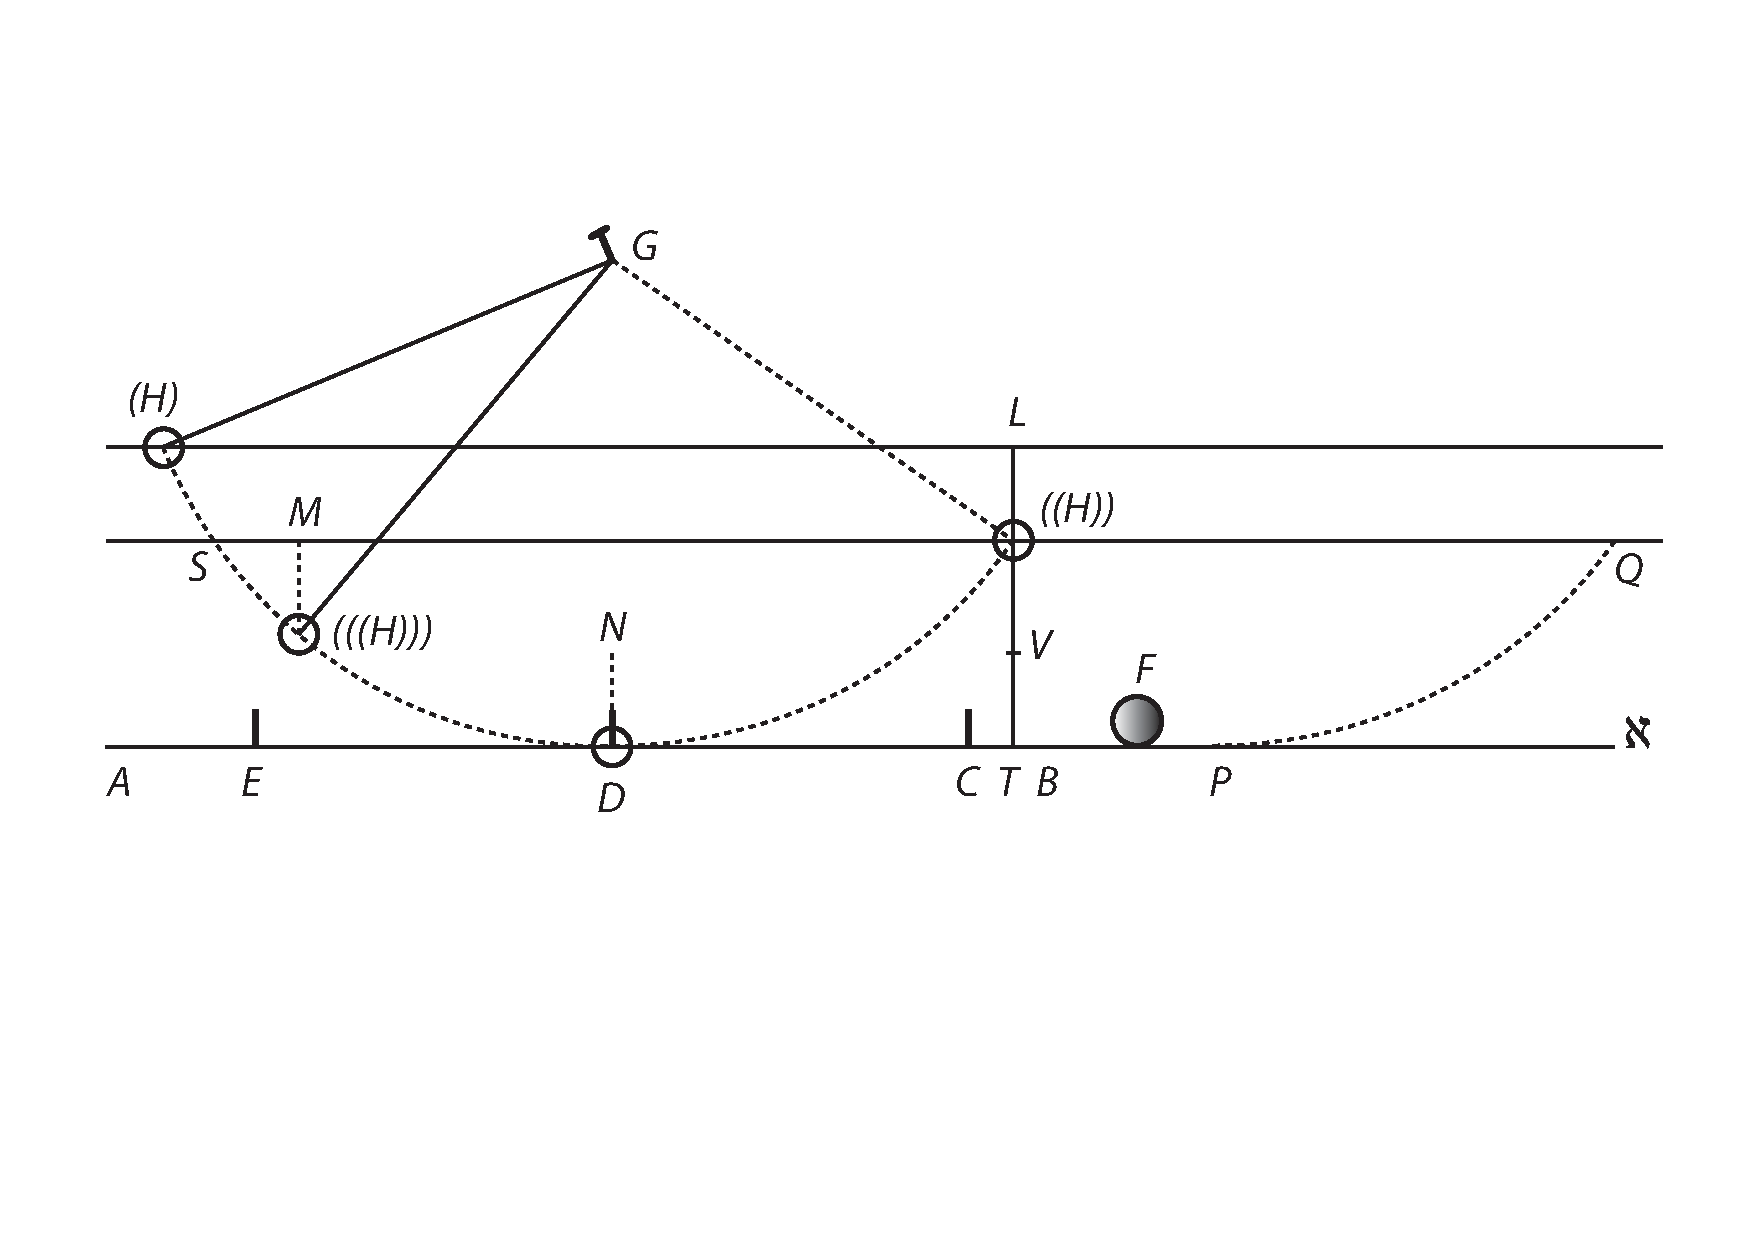
\includegraphics[trim = 17mm 60mm 5mm 35mm, clip, width=0.62\textwidth]{images/lh0351303_261r-d1.pdf}
   \noindent \centering [\textit{Fig. 1}]  % \caption{Bildbeschreibung}
    \end{wrapfigure}
\edtext{Cogitetur superficies $\displaystyle AB$}{\lemma{Cogitetur}\Bfootnote{\textit{(1)}\ planum $\displaystyle AB$ \textit{(2)}\ superficies $\displaystyle AB$ \textit{L}}} eminentiis \edtext{$\displaystyle C.$ $\displaystyle D.$ $\displaystyle E$}{\lemma{}\Bfootnote{$\displaystyle C.$ $\displaystyle D.$ $\displaystyle E$ \textit{erg.} \textit{L}}} consita, per aequalia intervalla \edtext{similiter}{\lemma{}\Bfootnote{similiter \textit{erg.} \textit{L}}} dispositis, calculi scilicet causa, ut aequaliter ubique aspera intelligatur[;] per eam incedere debet \edtext{corpus $\displaystyle F$ impetu aliquo}{\lemma{corpus $\displaystyle F$}\Bfootnote{\textit{(1)}\ quaesito impetu, vel \textit{(2)}\ impetu aliquo \textit{L}}},
quem utique vel ab alicujus gravis descensu, vel ab alicujus Elateris displosione nactum est. Quod eminentiam sibi occurrentem \edtext{$\displaystyle C$ elaterio instructam}{\lemma{}\Bfootnote{$\displaystyle C$ elaterio instructam \textit{erg.} \textit{L}}} deprimet, quantum satis est ad itineris libertatem, inque eo \edtext{opere aliquam virium}{\lemma{opere}\Bfootnote{\textit{(1)}\ certam virium q \textit{(2)}\ aliquam virium \textit{L}}} partem amittet, tantam scilicet \edtext{quantam elateri}{\lemma{quantam}\Bfootnote{\textit{(1)}\ elaterio \textit{(2)}\ elateri \textit{L}}} \edtext{$\displaystyle C$}{\lemma{}\Bfootnote{$\displaystyle C$ \textit{erg.} \textit{L}}} \edtext{contulit, quem}{\lemma{contulit,}\Bfootnote{\textit{(1)}\ quod \textit{(2)}\ quem \textit{L}}} transeundo subegit ac tetendit. Ut autem judicare liceat de quantitate virium amissarum, utendum est argumento meo solenni, quo Elementa Mechanicae \edtext{demonstro,}{\lemma{demonstro}\Cfootnote{?? Stelle nicht nachgewiesen.}} exposita motus \edtext{perennis interni impossibilitate}{\lemma{perennis}\Bfootnote{\textit{(1)}\ impossibilitate \textit{(2)}\ interni impossibilitate \textit{L}}}. Ponatur \edtext{scilicet pondus $\displaystyle H$ ex centro $\displaystyle G$ pendulum}{\lemma{scilicet}\Bfootnote{\textit{(1)}\ pendulum \textit{(2)}\ pondus $\displaystyle H$ ex centro  \textit{(a)}\ $\displaystyle D$ pend \textit{(b)}\ $\displaystyle G$ pendulum \textit{L}}}, quod ex altitudine $\displaystyle (H)$ descendens in itinere subigat superetque \edtext{elaterium $\displaystyle D$ et postea rursus ascendat in $\displaystyle ((H))$. Ducantur per puncta $\displaystyle (H).$ $\displaystyle ((H))$ rectae horizonti parallelae $\displaystyle (H)L.$ $\displaystyle ((H))M$ et ex puncto $\displaystyle ((H))$ perpendicularis sit $\displaystyle ((H))L$. Ajo}{\lemma{elaterium $\displaystyle D$}\Bfootnote{\textit{(1)}\ . Ajo \textit{(2)}\ et  postea [...] in $\displaystyle ((H))$ \textit{(a)}\  per punc \textit{(b)}\ . Ducantur [...] perpendicularis  \textbar\ sit \textit{erg.}\ \textbar\  $\displaystyle ((H))L$. Ajo \textit{L}}} rectam $\displaystyle ((H))L$ tantae esse altitudinis, quanta \edtext{est $\displaystyle DN$[,] ad quam}{\lemma{est}\Bfootnote{\textit{(1)}\ illa  \textit{(a)}\ in quam \textit{(b)}\ ad quam \textit{(2)}\ $\displaystyle DN$ ad quam \textit{L}}} scilicet Elaterium $\displaystyle DN$ \edtext{resiliens pondus $\displaystyle H$ sibi impositum}{\lemma{resiliens}\Bfootnote{\textit{(1)}\ rectam sibi impositam perpendi \textit{(2)}\  pondus [...] impositum \textit{L}}}\edtext{ ejaculando attollere possit}{\lemma{impositum}\Bfootnote{\textit{(1)}\ ejaculari possit \textit{(2)}\ ejaculando attollere possit \textit{L}}}.
Unde si ex [$\displaystyle ((H))$]\edtext{}{\Bfootnote{$\displaystyle H$ \textit{\ \ L \"{a}ndert Hrsg.}}} \edtext{redelabatur, in}{\lemma{redelabatur,}\Bfootnote{\textit{(1)}\ id \textit{(2)}\ in \textit{L}}} eodem obstaculo $\displaystyle D$ superando tantundem rursus virium amittet quantum ante, et ad altitudinem ascendet $\displaystyle (((H)))$. Unde si recta ducatur \edtext{$\displaystyle (((H)))M$}{\lemma{}\Bfootnote{$\displaystyle(((H)))M$ \textit{erg.} \textit{L}}} perpendicularis ad $\displaystyle ((H))M$ erit ea aequalis ipsi $\displaystyle DN$ vel $\displaystyle ((H))L$, atque ita porro continuatis penduli\protect\index{Sachverzeichnis}{pendulum} reciprocationibus altitudines ascensuum ab obstaculo arithmetice diminuentur. Idem ergo eveniet, \edtext{si pondus $\displaystyle H$}{\lemma{si}\Bfootnote{\textit{(1)}\ pendulum $\displaystyle H$ \textit{(2)}\ pondus $\displaystyle H$ \textit{L}}} per arcum solidum $\displaystyle (H)D$ descendere ibique in plano motum continuare, et in itinere obstaculum $\displaystyle C$ ipsi $\displaystyle D$ simile et aequali invenire ponamus; quo superato mox rursus per arcum solidum [$\displaystyle PQ$]\edtext{}{\Bfootnote{$\displaystyle DQ$\textit{\ \ L \"{a}ndert Hrsg.}}}, ipsi imaginario $\displaystyle D((H))$ similem \edtext{similiter positum}{\lemma{similiter}\Bfootnote{\textit{(1)}\ posita \textit{(2)}\ positum \textit{L}}} et aequalem denuo ascendat usque in $\displaystyle Q$. Cadet enim $\displaystyle Q$ in rectam $\displaystyle M((H))$ si opus est continuatam[,] eodem \edtext{modo si non assurgere post superatum obstaculum sed novum obstaculum aequalibus semper intervallis reperire intelligatur}{\lemma{modo}\Bfootnote{\textit{(1)}\ novis obstaculis aequalibus et similibus occurrentibus \textit{(2)}\ si non [...] intelligatur \textit{L}}}, et post aliquot obstacula \edtext{superata ponatur}{\lemma{superata}\Bfootnote{\textit{(1)}\ cogitetur \textit{(2)}\ ponatur \textit{L}}} sursum convertere motum[,] toties aberit a \edtext{puncto descensus $\displaystyle (H)$}{\lemma{puncto}\Bfootnote{\textit{(1)}\ $\displaystyle (H)$ descensu \textit{(2)}\ descensus $\displaystyle (H)$ \textit{L}}} altitudine $\displaystyle ((H))L$ quot sunt unitates in numero obstaculorum; adeoque si obstacula intelligantur infinita et infinite parva,
\edtext{et superficies $\displaystyle AB$ aequaliter aspera}{\lemma{et}\Bfootnote{\textit{(1)}\ corpus aequaliter  \textit{(a)}\ unitum \textit{(b)}\ asperum \textit{(2)}\ superficies [...] aspera \textit{L}}}
erunt deminutiones altitudinum resurgentis spatiis proportionales: Theorema ergo hoc erit: \edtext{Si grave}{\lemma{Si}\Bfootnote{\textit{(1)}\ corpus \textit{(2)}\ grave \textit{L}}} \edtext{in plano inclinato}{\lemma{grave}\Bfootnote{\textit{(1)}\ ex aliqua altitudine inclinate \textit{(2)}\ in plano inclinato \textit{L}}} descendens, motum \edtext{in plano}{\lemma{}\Bfootnote{in \textbar\ aliquo \textit{gestr.}\ \textbar\ plano \textit{L}}} horizontali \edtext{aequaliter aspero}{\lemma{}\Bfootnote{aequaliter aspero \textit{erg.} \textit{L}}} continuet aliquandiu et inde rursus sursum convertat, erunt diminutiones altitudinum
\edtext{resurgentis, a frictione factae plani horizontalis asperi ipsis longitudinibus}{\lemma{resurgentis,}\Bfootnote{\textit{(1)}\ spatiis  \textit{(a)}\ plani ipsis asperi  \textit{(b)}\ ipsis plani asperi \textit{(2)}\ a frictione [...] longitudinibus \textit{L}}}
proportionales. Porro hinc \edtext{jam habemus modum aestimandi etiam quantum celeritatis perdatur frictione}{\lemma{jam}\Bfootnote{\textit{(1)}\ sequitur friction \textit{(2)}\ habemus [...] frictione \textit{L}}}. \edtext{Nimirum  tantum celeritatis prima frictione quanta celeritate}{\lemma{Nimirum}\Bfootnote{\textit{(1)}\ quantum opus est celeri \textit{(2)}\  tantum celeritatis  \textit{(a)}\ primo ictu \textit{(b)}\ prima [...] celeritate \textit{L}}} pendulum ascendet per altitudinem ultimam [$\displaystyle L((H))$]\edtext{}{\Bfootnote{$\displaystyle LH$\textit{\ \ L \"{a}ndert Hrsg.}}}, seu quantam acquisivit descendendo ex $\displaystyle (H)$ ad $\displaystyle S$. Et generaliter si abstrahendo a \edtext{pendulo grave}{\lemma{}\Bfootnote{pendulo  \textbar\ solum \textit{gestr.}\ \textbar\ grave \textit{L}}} per rectam $\displaystyle L((H))T$ descendere libere intelligamus et in partes%\pend